\chapter{Interfaces}
\label{chap:interfaces}
Het doel van deze masterproef is het maken van een implementatie van GeoSPARQL in Comunica en te controleren of het hierbij mogelijk is om GeoSPARQL functionaliteiten te implementeren in deze \textit{query engine} die over verschillende heterogene data bronnen kan queryen. Hierbij worden de gegevens op de gebruikelijke manier opgehaald, maar worden de geospatiale relaties uitgerekend op de client-side. Hierbij moet gecontroleerd worden of dit mogelijk is bij de bronnen die momenteel door Comunica ondersteund worden. De belangrijkste bronnen zijn ``data dumps'', ``triple pattern fragment interfaces'' en ``sparql endpoints''. In de komende secties wordt besproken of dit mogelijk is en hoe dit werkt. De eerstvolgende sectie geeft echter een kort overzicht van de gebruikte dataset voor deze tests.

\section{Testset}
\label{sec:testset}
Bij de testset is ervoor gekozen om een oppervlakkige tekening te maken van België in een aangepaste schaal. Deze keuze is gemaakt om meerdere redenen. Om te beginnen laat deze aangepaste schaal zeer gemakkelijk toe om (als mens) vlakken te beschrijven. Aangezien dit een technisch en bovendien vooruitstrevend onderwerp is, is het handig om terug te keren naar een bekender terein. Daarom is de bekendheid van deze \textit{use case} meteen de tweede reden van deze keuze. Een derde reden is dat deze dataset eerder klein is, waardoor mogelijke fouten of onlogische oplossingen hierbij nogmaals getest worden. Ten slotte is dit ook de perfecte dataset voor het geven van demonstraties omdat deze set herkenbaar is voor het publiek. Een visualisatie van deze dataset is te zien in \figureref{fig:demoset}. De effectieve dataset is dan weer te vinden op GitHub Gist\footnote{https://gist.github.com/dreeki/e48bbe533a4b1191045b3652ff2c9c81}. Deze dataset is bovendien opgesplitst in vijf verschillende bestanden (namelijk: ``land'', ``gewest'', ``provincie'', ``weg'' en ``stad'') zodat deze dataset bruikbaar is voor het verifiëren of gefedereerd queryen nog steeds mogelijk is. Het geheel van deze testing wordt uitgevoerd in de testomgeving die besproken werd in \sectionref{sec:testomgeving}. Hierbij zorgt de \textit{execution log} ervoor dat alles duidelijk is hoe het geheel in zijn werk gaat.

\begin{figure}
    \centering
    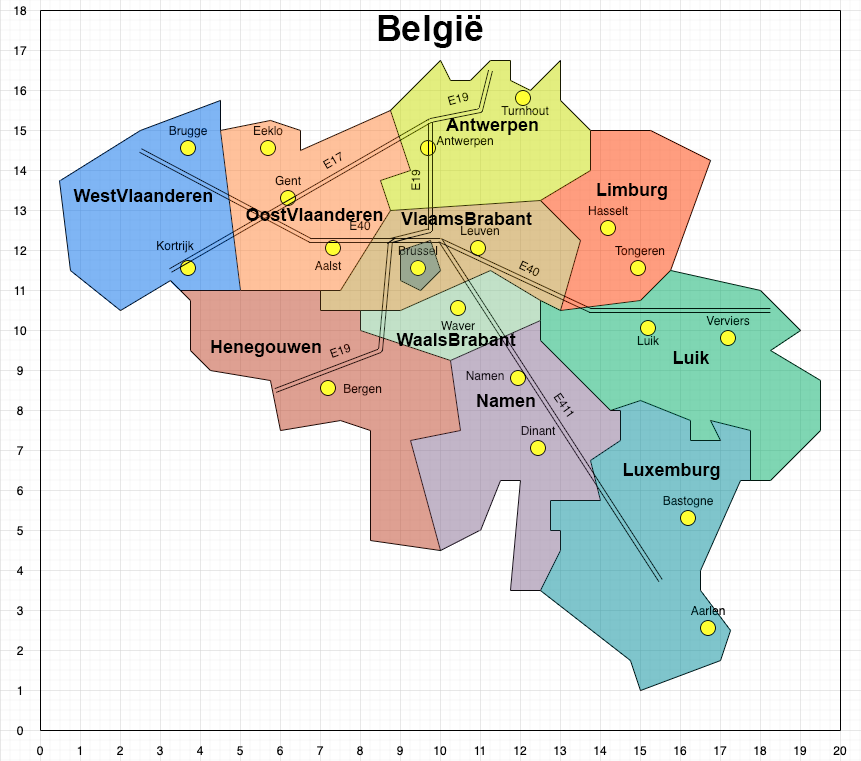
\includegraphics[width=\linewidth]{images/geosparql_demo.png}
    \caption{Testset voor het testen van de verschillende bronnen.}
    \label{fig:demoset}
\end{figure}


\subsection{queries}
Voor de uitvoering van de tests zijn verschillende queries opgesteld om mee te testen. In de testomgeving zelf kunnen hierbij vervolgens de bronnen aangepast worden naar de te testen bronnen. Het is echter wel nog op te merken dat de ontologieën bij de testomgeving reeds in code aangegeven werden. Bij gevolg worden deze niet opnieuw mee opgenomen in de geschreven query, maar in de achtergrond worden deze dus wel nog gebruikt.

\subsubsection{Query 1}
De eerste \textit{query} zoekt naar alle provincies die binnen Vlaanderen liggen. Om dit te kunnen doen zal de \textit{query engine} eerst de vorm van Vlaanderen zelf opzoeken. Daarna zal hij de vorm van alle provincies zoeken zodat hij met de ``sfContains'' functie van GeoSPARQL uiteindelijk kan filteren. Deze query is te zien in \listingref{listing:find_provinces_flanders}.

\begin{listing}[ht]
    \begin{minted}{sparql}
        SELECT ?f
        WHERE {
            gewest:Vlaanderen my:hasExactGeometry ?aGeom .
            ?aGeom geo:asWKT ?aWKT .
            ?f a my:Provincie .
            ?f my:hasExactGeometry ?fGeom .
            ?fGeom geo:asWKT ?fWKT .
            FILTER (geof:sfContains(?aWKT, ?fWKT))
        }
    \end{minted}
    \caption{Find all the provinces in Flanders.}
    \label{listing:find_provinces_flanders}
\end{listing}


\subsubsection{Query 2}
De tweede \textit{query} is zeer gelijkaardig aan de eerste, maar hier is één groot verschil. Deze \textit{query} zoekt naar alles dat binnen Vlaanderen ligt. Aangezien ``sfContains'' functie stelt dat een geospatiaal identieke vorm steeds binnen de andere ligt, zou deze query Vlaanderen zelf ook als een oplossing zien. Aangezien dit niet het verwachte resultaat is, wordt gebruik gemaakt van de negatie van de ``sameterm'' functie van SPARQL. Dit wijst er nogmaals op dat een werkende implementatie van SPARQL een vereiste is voor het maken van een GeoSPARQL implementatie. Deze query is te zien in \listingref{listing:find_everything_flanders}.

\begin{listing}[ht]
    \begin{minted}{sparql}
        SELECT ?f
        WHERE {
            gewest:Vlaanderen my:hasExactGeometry ?aGeom .
            ?aGeom geo:asWKT ?aWKT .
            ?f my:hasExactGeometry ?fGeom .
            ?fGeom geo:asWKT ?fWKT .
            FILTER (geof:sfContains(?aWKT, ?fWKT) && !sameterm(?aWKT, ?fWKT))
        }
    \end{minted}
    \caption{Find everything that's geospatially inside Flanders.}
    \label{listing:find_everything_flanders}
\end{listing}


\subsubsection{Query 3}
De derde query gaat dan weer over het vinden van de wegen en provincies die binnen België liggen. Deze query toont nogmaals aan hoe gelijkaardig SQL en SPARQL zijn. Deze query is te zien in \listingref{listing:find_provinces_roads_belgium}.

\begin{listing}[ht]
    \begin{minted}{sparql}
        SELECT ?f
        WHERE {
            land:België my:hasExactGeometry ?aGeom .
            ?aGeom geo:asWKT ?aWKT .
            {
                ?f a my:Provincie .
            }
                UNION
            {
                ?f a my:Weg .
            }
            ?f my:hasExactGeometry ?fGeom .
            ?fGeom geo:asWKT ?fWKT .
            FILTER (geof:sfContains(?aWKT, ?fWKT))
        }
    \end{minted}
    \caption{Find all the provinces and roads in Belgium.}
    \label{listing:find_provinces_roads_belgium}
\end{listing}


\subsubsection{Query 4}
Bij de vierde query worden alle wegen die door Oost-Vlaanderen gaan opgezocht. Dit zou bijvoorbeeld handig kunnen zijn wanneer iemand de snelwegen wil vinden die eenvoudig bereikbaar zijn vanuit Oost-Vlaanderen. Hierbij wordt de functie ``sfIntersects'' van GeoSPARQL gebruikt. Deze query is te zien in \listingref{listing:find_roads_passing_east_flanders}.

\begin{listing}[ht]
    \begin{minted}{sparql}
        SELECT ?f
        WHERE {
            prov:OostVlaanderen my:hasExactGeometry ?aGeom .
            ?aGeom geo:asWKT ?aWKT .
            ?f a my:Weg .
            ?f my:hasExactGeometry ?fGeom .
            ?fGeom geo:asWKT ?fWKT .
            FILTER (geof:sfIntersects(?aWKT, ?fWKT))
        }
    \end{minted}
    \caption{Find all the roads that pass through East-Flanders.}
    \label{listing:find_roads_passing_east_flanders}
\end{listing}


\subsubsection{Query 5}
De vijfde query toont aan dat het mogelijk is om manueel een vorm te voorzien om op te filteren. Deze vorm staat (bij de aangepaste schaal) voor de \textit{bounding box} van Vlaams-Brabant en Waals-Brabant. Deze query zal alles weergeven dat zich binnen deze vorm bevindt. Voor de verandering wordt hier de ``sfWithin'' functie van GeoSPARQL gebruikt, maar dit zou evengoed mogelijk zijn met de ``sfContains'' functie. Deze query is te zien in \listingref{listing:find_everything_bounding_box}.

\begin{listing}[ht]
    \begin{minted}{sparql}
        SELECT ?f
        WHERE {
            ?f my:hasExactGeometry ?fGeom .
            ?fGeom geo:asWKT ?fWKT .
            FILTER (geof:sfWithin(?fWKT, '''Polygon((7 9.25, 13.5 9.25, 13.5 13.25, 
            7 13.25, 7 9.25))'''^^geo:wktLiteral))
        }
    \end{minted}
    \caption{Find everything inside the bounding box of Brabant.}
    \label{listing:find_everything_bounding_box}
\end{listing}




\todo{misschien nog extra queries} 
\newpage
\section{Data dump}
\label{sec:data-dump}
De eerste bron om te controleren, wordt gebruikt als baseline. Dit is de ``data dump''. Dit is een gewoon bestand in RDF formaat dat door de \textit{query engine} opgehaald (lees gedownload) wordt. Vervolgens wordt het door de \textit{query engine} gecontroleerd of het effectief wel een bestandsbron is. Eenmaal dit voldaan is, worden steeds de kleinste patronen gezocht die voldoen aan de bron. Dit is nodig omdat de \textit{query engine} zo op de meest performante manier de \textit{joins} kan uitvoeren. Zo kan ten slotte de filter-functie de overbodige oplossingen weghalen. Deze filter-functie is voorzien door GeoSPARQL. Bovendien voorziet Comunica functionaliteiten om data-entiteiten uit de databron te extraheren, wat hier gebeurt op de client. Over deze entiteiten moet een filter functie geëvalueerd kunnen worden. Hierdoor is het mogelijk om data dumps te queryen met GeoSPARQL. Aangezien data dumps letterlijk bestanden zijn zonder een eigen voorziening van logica, is het triviaal dat dit afgehandeld moet kunnen worden. De data dump wordt daarom de \textit{baseline} van dit onderzoek, waarbij er gepoogd wordt om dezelfde resultaten bij andere bronnen ook te behalen.

Bij het testen van de data dump worden de GitHub Gist bestanden (zie \sectionref{sec:testset}) rechtstreeks gebruikt. Hier is geen enkel ander programma dat als aanspreekpunt gebruikt wordt. Hierbij is dus ook duidelijk dat het beschreven proces van hierboven correct doorlopen is. Dit is bovendien de manier van werken die gebruikt is bij het maken en testen van de implementatie. 
\newpage
\section{Triple pattern fragment interface}
\label{sec:impl_tpf_interface}
De volgende bron is de ``triple pattern fragment interface''. Dit is een server die tussen de op te vragen bestanden (dus de effectieve gegevens) en de client staat. Deze server zal ervoor zorgen dat het niet langer nodig is om alle data op te halen, maar in de plaats zal de server de SPARQL query splitsen in verschillende triple pattern fragment requests. Deze vragen alle triples die voldoen aan een enkel tripple pattern fragment en \textit{joinen} dan de resultaten op de client. De filtering gebeurt daarna ook op de client.

Net zoals bij de data dump (zie \sectionref{sec:data-dump}) vraagt de \textit{query engine} de bron op. Hierbij zal hij de bron identificeren als een ``qpf source'', wat staat voor ``Quad pattern fragment''. Dit is eigenlijk de \textit{triple pattern fragment} met hierbij een extra veld (graph) toegevoegd, maar hier wordt niet verder op in gegaan. Vervolgens begint de \textit{query engine} de query op de splitsen in TPF queries, zodat deze TPF queries geoptimaliseerd kunnen worden in een volgorde die gebaseerd is op de initiële count query. Hierna worden deze één voor één uitgevoerd. Zo zal hij vervolgens de kleinste patronen opvragen, zodat de correcte informatie opgevraagd kan worden met hierbij een minimale hoeveelheid aan overbodige informatie mee te krijgen. Dit is enkel mogelijk dankzij de TPF interface. Dankzij deze manier van werken kan wederom de uiteindelijke filtering van de \textit{queries} louter op de client-side gebeuren.

Voor het opzetten van deze test is gebruik gemaakt van de ``Linked Data Fragments Server''. Deze bouwt een TPF interface op boven een set van bronbestanden, waarvoor opnieuw de bestanden van GitHub Gist gebruikt zijn, net zoals bij de data dump. Op deze manier is ook verzekerd dat er met dezelfde gegevens gewerkt wordt. 

Als kleine opmerking kan nog vermeld worden dat een TPF interface gebruikt wordt voor twee redenen. Ten eerste hoeft de client zo niet alle data te downloaden, maar kan de server slechts een fragment (vandaar de naam, deze komt eigenlijk van ``Linked Data Fragments'') van deze data teruggeven. De tweede reden is dat deze filtering meestal (= niet in alle gevallen) zorgt voor een verbeterde performantie. Bij het testen was dit echter niet terug te vinden. Zo blijkt het uitvoeren van de queries met de data dump sneller te gaan dan met de TPF interface. Hier is echter een logische verklaring voor. De datasets dit gebruikt zijn, zijn relatief gezien kleine datasets. Bovendien bevatten deze enkel de noodzakelijke gegevens, waardoor de dataset volledig nodig is voor het uitvoeren van de query. Hierdoor kan er niet genoten worden van de voordelen van de TPF interface, maar wordt enkel de extra \textit{overhead} waargenomen. Dit gaat echter buiten de \textit{scope} van deze scriptie, daarom werd hier verder geen onderzoek naar gedaan, noch benchmarking van de performantie. Dit is eerder een opmerking bij de ondervindingen. 
\newpage
\section{SPARQL endpoint}
\label{sec:impl_sparql_endpoint}
De laatste bron om te testen is meteen de moeilijkste. Bij het SPARQL endpoint is het de bedoeling dat een GeoSPARQL query uitgevoerd kan worden door de gegevens op te vragen aan dit SPARQL endpoint. Comunica zelf is gemaakt om queries uit te voeren over RDF bronnen, wat het zeer handig maakt om SPARQL queries uit te voeren. Hierdoor lijkt het logisch om de query in zijn geheel door te sturen in het geval van een SPARQL endpoint als bron. Dit SPARQL endpoint is namelijk in staat om volledig automoon een antwoord te geven op de query. Dit is echter niet hoe het in zijn werk gaat. Eén van de redenen hiervoor is dat gefedereerd queryen zo niet mogelijk zou zijn wanneer er naast het SPARQL endpoint nog een andere bron zou zijn. Zo moet de samenvoegingen van de antwoorden op de client-side gebeuren. 

Bij een SPARQL endpoint zal de \textit{query engine} de verschillende RDF triples van de query overlopen. Dit doet hij in twee stappen. De eerste stap is een ``count'' zodat hij weet hoeveel RDF triples van de bron overeen komen met de RDF triples van de query. Dit wordt gedaan zodat de \textit{query engine} weet welke volgorde optimaal is om de data op te halen, zodat hij dit optimaal kan joinen. De tweede stap is het effectieve ophalen van het resultaat, waarbij hij dus alle antwoorden vraagt die voldoen aan slechts één RDF triple van de query. Wanneer dit voor alles gedaan is zoekt hij het kleinste patroon, zodat hij vervolgens de matchende RDF triples kan ophalen. Het kleinste patroon wordt gekozen om het aantal matchende resultaten te minimaliseren voor performantie redenen.

Zo wordt uiteindelijk alle benodigde informatie uit het SPARQL endpoint systematisch opgehaald, zodat de filter bij de oorspronkelijke query onafhankelijk van de bronnen kan uitgevoerd worden. Dit betekent ook dat de filter functies steeds dezelfde implementatie hebben (namelijk deze van de \textit{query engine} op de client, niet deze van de bron). Dit laat echter ook toe om te filteren met de GeoSPARQL functies. Dankzij deze werkwijze is het dus effectief mogelijk om de GeoSPARQL functionaliteit toe te passen bij het opvragen aan een SPARQL endpoint. 
\newpage